\chapter{Theoretische Grundlagen}

\section{Einführung in Künstliche Intelligenz und NLP}
\subsection{Historischer Überblick über NLP und dessen Bedeutung}

Natural Language Processing (NLP) hat seine Ursprünge in den 1950er Jahren, als die erste maschinelle Übersetzung durchgeführt wurde. Seitdem hat sich NLP als wesentlicher Bereich der Künstlichen Intelligenz etabliert. Seine Bedeutung zeigt sich in Anwendungen wie maschineller Übersetzung, Sprachassistenten und automatischer Textzusammenfassung. Die Entwicklung leistungsfähiger neuronaler Netzwerke hat NLP revolutioniert und neue Anwendungsbereiche erschlossen.

\subsection{Grundlagen neuronaler Netze und LSTMs (Long Short-Term Memory)}

Neuronale Netze sind rechnerische Modelle, die von der Struktur biologischer Gehirne inspiriert sind. Sie bestehen aus Schichten von Neuronen, die Informationen durch gewichtete Verbindungen weitergeben. LSTMs sind eine spezielle Art von rekurrenten neuronalen Netzen (RNNs), die speziell für die Verarbeitung und Speicherung von sequenziellen Daten wie Text entwickelt wurden. Sie adressieren das Problem des Verschwindens von Gradienten, indem sie "Gates" einführen, die den Informationsfluss steuern.

\subsection{Erklärung von neuronalen Netzen von Grund auf}

\textbf{Grundaufbau eines neuronalen Netzes:} Neuronale Netze bestehen aus verbundenen Knoten, die als Neuronen bezeichnet werden. Diese Neuronen sind in Schichten organisiert:

\begin{itemize}
    \item \textbf{Eingabeschicht:}
    \begin{itemize}
        \item  Nimmt die Eingabedaten auf.
    \end{itemize}
    \item \textbf{Verborgene Schichten:}
    \begin{itemize}
        \item  Verarbeiten der Daten durch gewichtete Verbindungen.
    \end{itemize}
    \item \textbf{Ausgabeschicht:}
    \begin{itemize}
        \item  Liefert die Vorhersagen oder Ergebnisse des Netzes.
    \end{itemize}
\end{itemize}

\textbf{Mathematische Beschreibung eines Neurons:} Ein Neuron nimmt mehrere Eingaben \(x_1, x_2, \dots, x_n\) entgegen und berechnet eine gewichtete Summe:
\[
z = w_1 x_1 + w_2 x_2 + \dots + w_n x_n + b = \mathbf{w}^T \mathbf{x} + b
\]
wobei \( \mathbf{w} \) die Gewichte, \( \mathbf{x} \) die Eingaben und \( b \) der Bias sind. Das Ergebnis wird durch eine Aktivierungsfunktion \( \phi \) transformiert:
\[
a = \phi(z)
\]
Gängige Aktivierungsfunktionen sind:
\begin{itemize}
    \item \textbf{Sigmoid:} \( \phi(z) = \frac{1}{1 + e^{-z}} \)
    \item \textbf{ReLU:} \( \phi(z) = \max(0, z) \)
    \item \textbf{Tanh:} \( \phi(z) = \frac{e^z - e^{-z}}{e^z + e^{-z}} \)
\end{itemize}

\textbf{Architekturen und Trainingsprinzipien:} Das Netz wird trainiert, indem ein Fehlermaß (z. B. Mean Squared Error, Cross-Entropy) minimiert wird. Hierbei wird Backpropagation verwendet, um Gradienten der Gewichte zu berechnen:
\begin{enumerate}
    \item \textbf{Vorwärtsdurchlauf:} Eingaben durch das Netz leiten und Fehler berechnen.
    \item \textbf{Rückwärtsdurchlauf:} Gradienten des Fehlers berechnen (Gradientenabstieg).
    \item \textbf{Gewichtsupdate:} 
    \[
    w_i \leftarrow w_i - \eta \frac{\partial L}{\partial w_i}
    \]
    wobei \( \eta \) die Lernrate und \( L \) der Verlust ist.
\end{enumerate}

\textbf{Python-Beispiel: Einfaches neuronales Netz:}
\begin{lstlisting}[language=Python, caption={Einfaches neuronales Netz in PyTorch}]
import torch
import torch.nn as nn
import torch.optim as optim

class SimpleNN(nn.Module):
    def __init__(self, input_size, hidden_size, output_size):
        super(SimpleNN, self).__init__()
        self.fc1 = nn.Linear(input_size, hidden_size)
        self.relu = nn.ReLU()
        self.fc2 = nn.Linear(hidden_size, output_size)

    def forward(self, x):
        x = self.fc1(x)
        x = self.relu(x)
        x = self.fc2(x)
        return x

# Hyperparameter
input_size = 3
hidden_size = 5
output_size = 2
learning_rate = 0.01

# Modell, Verlustfunktion und Optimierer
model = SimpleNN(input_size, hidden_size, output_size)
criterion = nn.MSELoss()
optimizer = optim.SGD(model.parameters(), lr=learning_rate)

# Beispieltraining
inputs = torch.tensor([[1.0, 2.0, 3.0]], requires_grad=True)
targets = torch.tensor([[0.0, 1.0]])

for epoch in range(100):
    outputs = model(inputs)
    loss = criterion(outputs, targets)
    optimizer.zero_grad()
    loss.backward()
    optimizer.step()

print(f"Final Loss: {loss.item()}")
\end{lstlisting}

\subsection{Relevante mathematische Konzepte}
\textbf{Backpropagation:} Dieses Verfahren wird verwendet, um die Gewichte eines neuronalen Netzes durch Minimierung eines Fehlermaßes zu aktualisieren. Der Fehler wird rückwärts durch das Netz propagiert.

\textbf{Softmax:} Diese Funktion normalisiert die Ausgaben eines neuronalen Netzes zu einer Wahrscheinlichkeitsverteilung, die für Klassifikationsprobleme geeignet ist. Mathematisch ist sie definiert als:
\[
\text{Softmax}(z_i) = \frac{e^{z_i}}{\sum_{j=1}^N e^{z_j}}
\]

\textbf{Cross-Entropy-Loss:} Ein Verlustmaß, das häufig bei Klassifikationsproblemen verwendet wird. Es berechnet den Unterschied zwischen der vorhergesagten Wahrscheinlichkeitsverteilung und der tatsächlichen Verteilung:
\[
L = - \sum_{i=1}^N y_i \log(\hat{y}_i)
\]

\section{Mathematische Modelle für NLP}

\subsection{Tokenization und Vektorisierung}
Die Tokenisierung zerlegt Text in kleinere Einheiten wie Wörter oder Subwörter. Diese Tokens werden durch Vektorisierung in numerische Darstellungen umgewandelt, die von neuronalen Netzen verarbeitet werden können. Methoden wie Bag of Words und Word Embeddings (z. B. Word2Vec, GloVe) sind gängige Ansätze zur Vektorisierung.

\subsection{Funktionsweise und mathematische Formulierung von LSTMs}

Ein LSTM besteht aus Zellen, deren interne Zustände durch drei Haupt-Gates gesteuert werden: das Eingabe-Gate, das Vergessens-Gate und das Ausgabe-Gate. Diese Gates nutzen Aktivierungsfunktionen wie die Sigmoid- und Tanh-Funktion, um Informationen selektiv zu speichern oder zu löschen. Mathematisch kann ein LSTM wie folgt beschrieben werden:
\[
\begin{aligned}
\text{Vergessens-Gate:} & \quad f_t = \sigma(W_f x_t + U_f h_{t-1} + b_f) \\
\text{Eingabe-Gate:} & \quad i_t = \sigma(W_i x_t + U_i h_{t-1} + b_i) \\
\text{Zustandsaktualisierung:} & \quad \tilde{C}_t = \tanh(W_c x_t + U_c h_{t-1} + b_c) \\
\text{Zellzustand:} & \quad C_t = f_t \odot C_{t-1} + i_t \odot \tilde{C}_t \\
\text{Ausgabe-Gate:} & \quad o_t = \sigma(W_o x_t + U_o h_{t-1} + b_o) \\
\text{Aktivierung:} & \quad h_t = o_t \odot \tanh(C_t)
\end{aligned}
\]

\subsection{Erklärung der Implementierungsschritte in PyTorch}
Die Implementierung eines LSTM in PyTorch beginnt mit der Definition des Modells, gefolgt von der Erstellung einer Vorwärts-Pass-Methode. PyTorch stellt leistungsstarke Funktionen für die Backpropagation und Optimierung bereit. Ein Beispiel für ein LSTM-Modell in PyTorch wurde in dieser Arbeit detailliert beschrieben. Jedoch sollte angemerkt werden, dass LSTMs nur im Zusammenhang mit CoreML verwendent worden sind.


% Beispielgraph (LSTM):
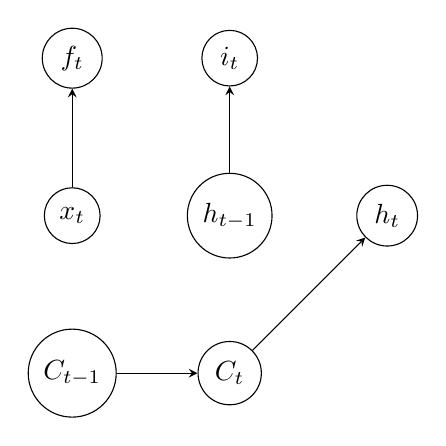
\begin{tikzpicture}[->, >=stealth, node distance=2cm]
    \node (xt) [circle, draw] {$x_t$};
    \node (ht_1) [circle, draw, right of=xt] {$h_{t-1}$};
    \node (ft) [circle, draw, above of=xt] {$f_t$};
    \node (it) [circle, draw, above of=ht_1] {$i_t$};
    \node (ct_1) [circle, draw, below of=xt] {$C_{t-1}$};
    \node (ct) [circle, draw, below of=ht_1] {$C_t$};
    \node (ht) [circle, draw, right of=ht_1] {$h_t$};

    % Arrows
    \draw [->] (xt) -- (ft);
    \draw [->] (ht_1) -- (it);
    \draw [->] (ct_1) -- (ct);
    \draw [->] (ct) -- (ht);
\end{tikzpicture}

\chapter{Implementierung}


\section{Trainingspipeline und Datenaugmentation}
% Details zum Training und zur Datenverarbeitung

\section{Modelltransformation für Core ML}
% Konvertierung des Modells von PyTorch zu Core ML

\section{Eigene Entwicklungen in Swift}
% Details zur Swift-ML-Library

\chapter{Ergebnisse}
\section{Evaluierung der Modellleistung}
% Ergebnisse und deren Analyse

\section{Vergleich von PyTorch- und Core ML-Implementierungen}
% Vergleich und Diskussion

\chapter{Fazit und Ausblick}
\section{Zusammenfassung}
% Kurze Zusammenfassung der Arbeit

\section{Limitationen und zukünftige Arbeiten}
% Mögliche Verbesserungen und Ausblick

\chapter{Anhang}
\section{Codeausschnitte}


\section{Zusätzliche technische Details}
% Weitere Anhänge und technische Informationen


